%****************************************************************************
%** Copyright 2002 by Lukas Ruf, ruf@topsy.net
%** Information is provided under the terms of the
%** GNU Free Documentation License http://www.gnu.org/copyleft/fdl.html
%** Fairness: Cite the source of information, visit http://www.topsy.net
%****************************************************************************
%****************************************************************************
%** Last Modification: 2005-07-11 1600
%** 2005-07-11	Bernhard Tellenbach
%**							This is an addapted version of the Introduction.tex file
%**							Added table example (footnotes,multicolumn)
%**							Examples for different text sizes
%**							Updated eps file inclusion example for use with graphicx pkt. 
%****************************************************************************

\chapter{\label{chapter2}Background}

In this chapter, we give a brief overview of BGP in \ref{chapter2:BGP} and explain the problem of long convergence time upon remote failure in BGP. We highlight the architecture and key insights of both iSDX and Swift in \ref{chapter2:iSDX} and \ref{chapter2:Swift}, respectively. The architecture of both frameworks are very similar, they are based on an SDN switch, an SDN controller and a route server. In the next chapter, we explain how these similarities can be put to use in the implementation.

\section{\label{chapter2:BGP}BGP}

The Border Gateway Protocol (BGP) allows autonomous systems to exchange routing information with each other. The routing information is communicated on a per prefix basis using BGP updates. BGP updates contain attributes. Attributes are the prefix, the next hop and the \\
AS-path the packet will traverse, if packets are sent via this route. There are two types of updates, announcements and withdraws. Announcements inform that the prefix can be reached via this route and withdraws inform that the previously announced prefix cannot be reached via this route anymore. 

Upon receiving a BGP update routers make a routing decision using the attributes of the BGP update and then send updates to their peers. Routers only send announcements with their own best route to the prefix and if the routers do not know a route to the prefix they send withdraws.

Convergence time in BGP upon remote failure can be slow.
This is because of the way updates propagate trough the network. Changes are only passed on once routers have finished computing the best route to the prefix. Only once all the updates have reached a router and it has finished the best path computation for all the updates, has the router converged. Meaning the router is able to make sure packets do not get sent into a loop or to a black hole anymore. The convergence time of a router is lower bounded by the time it takes for all the information/updates to be received. Because all routers before also have to process  the updates, the convergence time increases the further away the failure takes place. 


\section{\label{chapter2:iSDX}iSDX}

The iSDX is an Internet exchange point enhanced with a software defined networking (SDN) switch and a SDN controller.
An Internet exchange point (IXP) is a physical location where multiple autonomous systems meet to exchange traffic and BGP routes. An exchange point provides a fabric for the networks to interconnect. Each network attaches with one or multiple routers to this fabric. To reduce the burden on the network operators, Internet exchange points often provide a route server. Thanks to the route server, each border router only has to peer with the route server instead of all other participants. This allows participants to receive BGP updates from all other participants. However, even though many different routes might be available for a single prefix, participants of a traditional IXP can only use a single route per prefix.

The iSDX allows its participants to not only make use of these additional routes, but also gives the participants  more fine-grained control over the routing decisions. A participant connects to the iSDX as if it were a traditional IXP and is able to specify special policies that allow the participant to use multiple routes at once and control routing beyond the prefix.

We first show the iSDX architecture in \ref{chapter2:iSDX:iSDX_architecture}, explain the different policies and their capabilities in \ref{chapter2:iSDX:policies} and how the iSDX features are implemented using a virtual next hop and repurposing the destination mac address in \ref{chapter2:iSDX:VNH_VMAC}.

\subsection{\label{chapter2:iSDX:iSDX_architecture}iSDX Architecture}
\begin{figure}[h]
\center
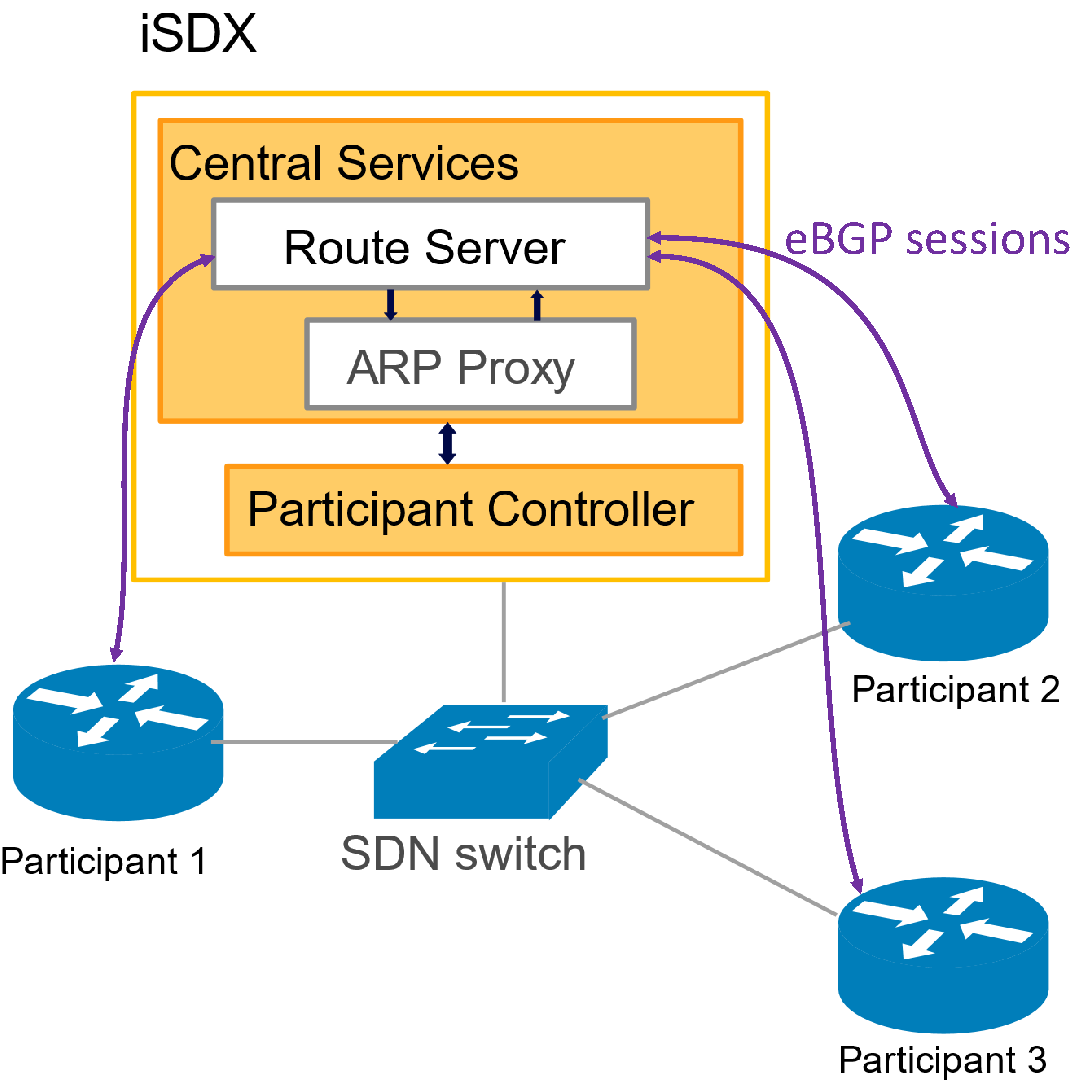
\includegraphics[scale = 0.3]{Figures/isdx_architectur_cropped.pdf}
\caption{iSDX architecture}
\end{figure}

The iSDX architecture consists of two main parts: \emph{(i)} the central services and \emph{(ii)} the participant controller.

The Central Services has two tasks. \emph{(i)} It collects all BGP updates and ARP queries centrally and forwards them to the corresponding participant controller. \emph{(ii)} It makes sure that BGP connection, default forwarding and ARP traffic is correctly handled by installing flow rules.

Every participant has its own participant controller. This allows each participant to make its own best path decision. The participant controller receives and processes BGP updates from the central route server. Every participant controller has a local routing information base (RIB), which keeps track of all the received routes, currently used routes and routes advertised to other participants. It takes care of the virtual next hop (VNH) and virtual MAC address (VMAC) assignment. It handles ARP requests and sends out gratuitous ARP replies. Before BGP updates get sent to the participants border router they are processed by the participant controller. It also installs all the flow rules which are necessary for its policies to be enforced.

\subsection{\label{chapter2:iSDX:policies}Policies}
Policies allow a participant to specify forwarding behavior which deviates from the default best path forwarding. They can be specified on any part of the header. Policies are implemented as flow rules that the participants controller programs into the SDN switch. Two types of policies exist: \emph{(i)} outbound policies that handle all out-going traffic and \emph{(ii)} inbound policies that handle all incoming traffic.

\paragraph{\label{chapter2:iSDX:policies:outbound policies}Outbound Policies:}
Outbound policies let participants direct packets going from themselves to the iSDX. They allow the participants to forward packets onto another path than the best path. An example of an outbound policy is shown in Figure~\ref{fig:isdx_policies}, where participant \emph{A} has defined two outbound policies \emph{X} and \emph{Y} directing traffic away from the best path to either one of the other two participants.

\paragraph{\label{chapter2:iSDX:policies:inbound policies}Inbound Policies:}
Inbound policies allow participants to specify how incoming packets are handled. In effect they allow the participant to choose to which of his own routers packets from the iSDX get sent to. An example of an inbound policy is shown in Figure~\ref{fig:isdx_policies}, where participant C has defined two inbound policies \emph{P} and \emph{Q} directing traffic to either one of its routers depending on the destination port. 

\begin{figure}[h]
\center
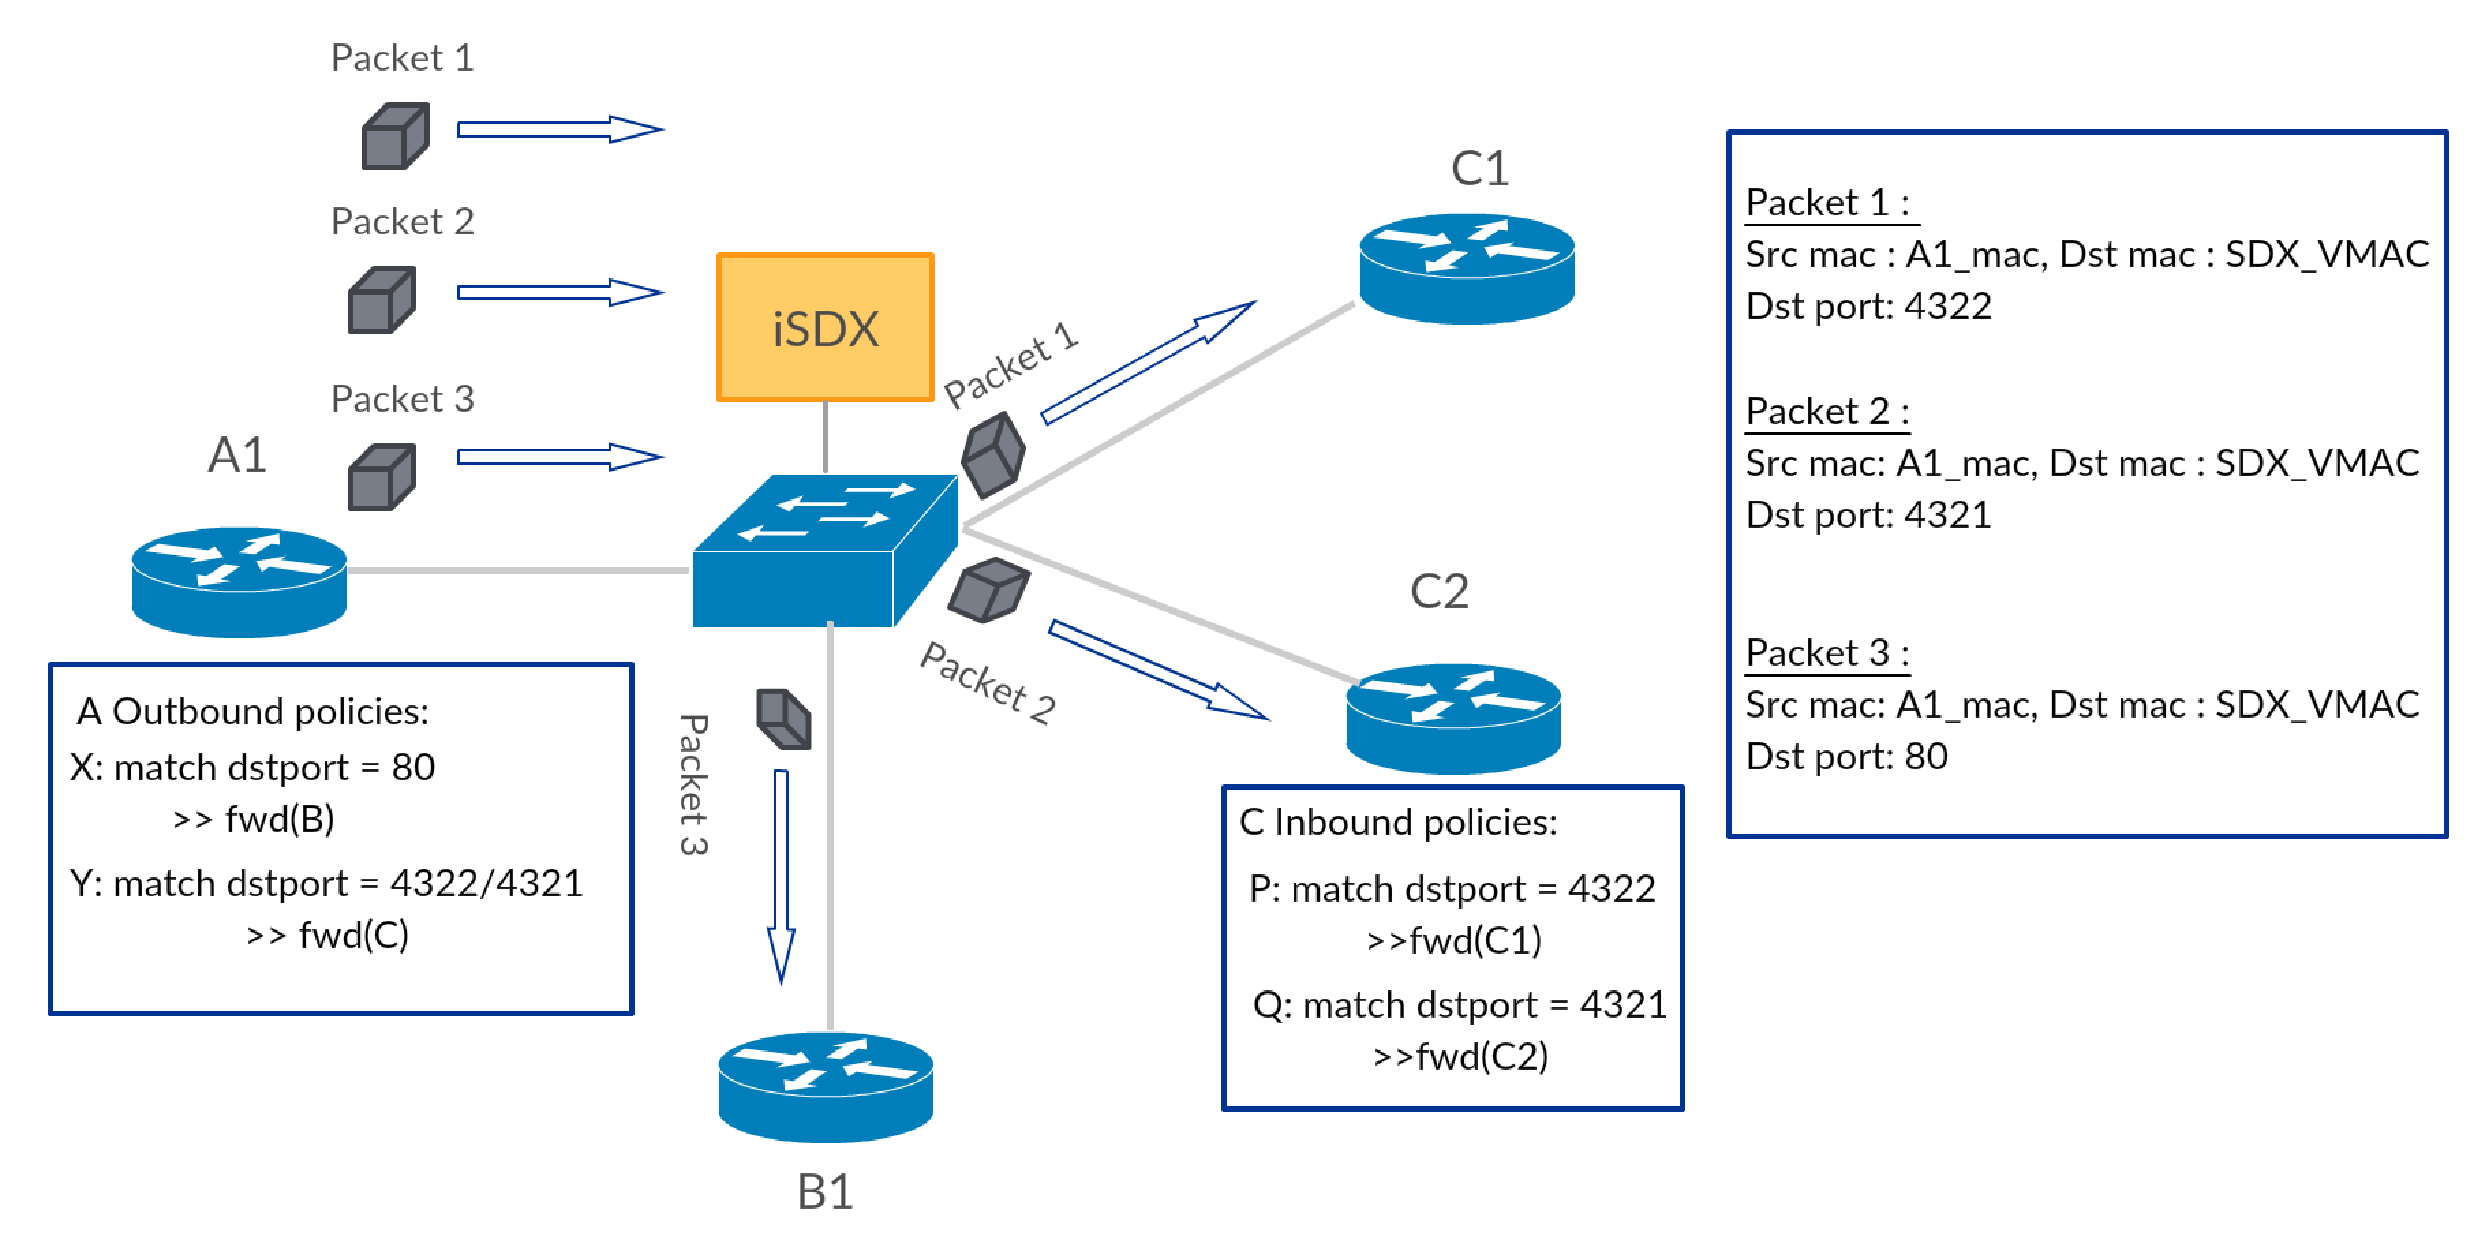
\includegraphics[scale = 0.31]{Figures/sdx_policies.pdf}
\caption{Example of outbound and inbound policies at an iSDX connected to three participants}
\label{fig:isdx_policies}
\end{figure}
  

\subsection{\label{chapter2:iSDX:VNH_VMAC}Virtual Next Hop, Virtual MAC Address}


Note that when specifying a policy, the network operator does not have to take into account whether the specified destination  is actually able to handle that traffic. Some policies might direct packets to participants that did not advertise the prefix to that participant or simply do not know a route to the prefix. Participants are not restricted when defining outbound policies. This is a problem because outbound policies can end up violating BGP advertisements. It is not possible to require participants to only specify feasible policies as the routing information is quite volatile and network operators would constantly need to update their policies to make sure none of the traffic is sent to a black hole. 

The iSDX solves this problem by attaching additional information to each packet. This additional information is embedded into the destination MAC address, transforming the destination MAC addresses of packets traversing the SDN switch into a Virtual Mac Address (VMAC).
In the VMAC the participant controller encodes the participants advertising the prefix of the packet and the BGP best next hop participant for this prefix. The first part is used every time a outbound policy is applied. The outbound policy checks if the participant the outbound policy is sending packets to has advertised the prefix. The second part is used if the packet does not match any outbound policy. Default rules in the SDN switch match on the best next hop participant and send the packet to this participant.

Each border router replaces the destination MAC address with the corresponding VMAC before sending a packet to the iSDX fabric. It is possible to assign this task to the participant's border routers using the next hop attribute in the BGP announcement. Every prefix is assigned a virtual next hop (VNH) that maps to a VMAC. Before sending BGP updates to its border routers the participant controller sets the next hop attribute to the VNH corresponding to the prefix of the update.  When a packet arrives at the border router it checks its routing table and finds the next hop, in this case the VNH. The border routers learn the VMAC of the VNHs via ARP. The border router broadcasts a ARP request for the VNH which is received by the ARP proxy, forwarded to the corresponding participant controller and replied to with the corresponding VMAC.

Figure~\ref{fig:isdx_vmac} shows the VNHs and VMACs used by participant A.

\begin{figure}[h]
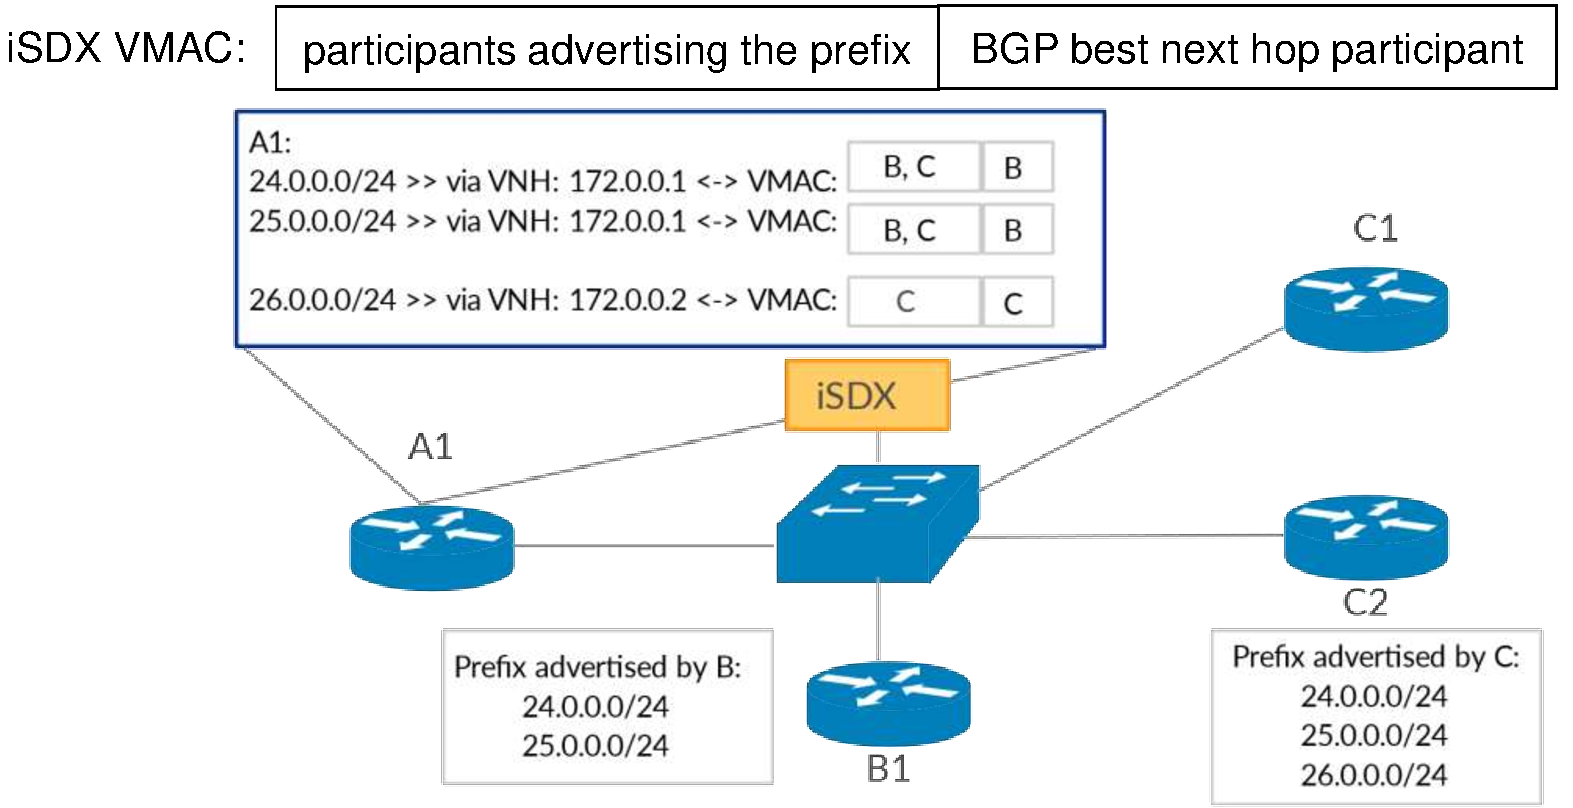
\includegraphics[scale = 0.4]{Figures/sdx_vmac2_cropped.pdf}
\caption{Example of the VMAC at an iSDX connected to three participants}
\label{fig:isdx_vmac}
\end{figure}

\newpage

\section{\label{chapter2:Swift}Swift}

Swift is a prediction and fast reroute (FR) framework which improves the convergence time of a BGP speaking router upon remote failures. Swifts prediction relies on the fact that the cause of a burst of withdrawals can be predicted before receiving all the withdrawals using the attributes of the already received withdrawals.

In this section, we first show the Swift architecture in \ref{chapter2:Swift:Architecture_SWift}, explain how Swift is able to reduce the convergence time of a router in \ref{chapter2:Swift:BPA} and explain the encoding in \ref{chapter2:Swift:encoding_of_routing_information}.

\subsection{\label{chapter2:Swift:Architecture_SWift}Architecture}

\begin{figure}[h]
\center
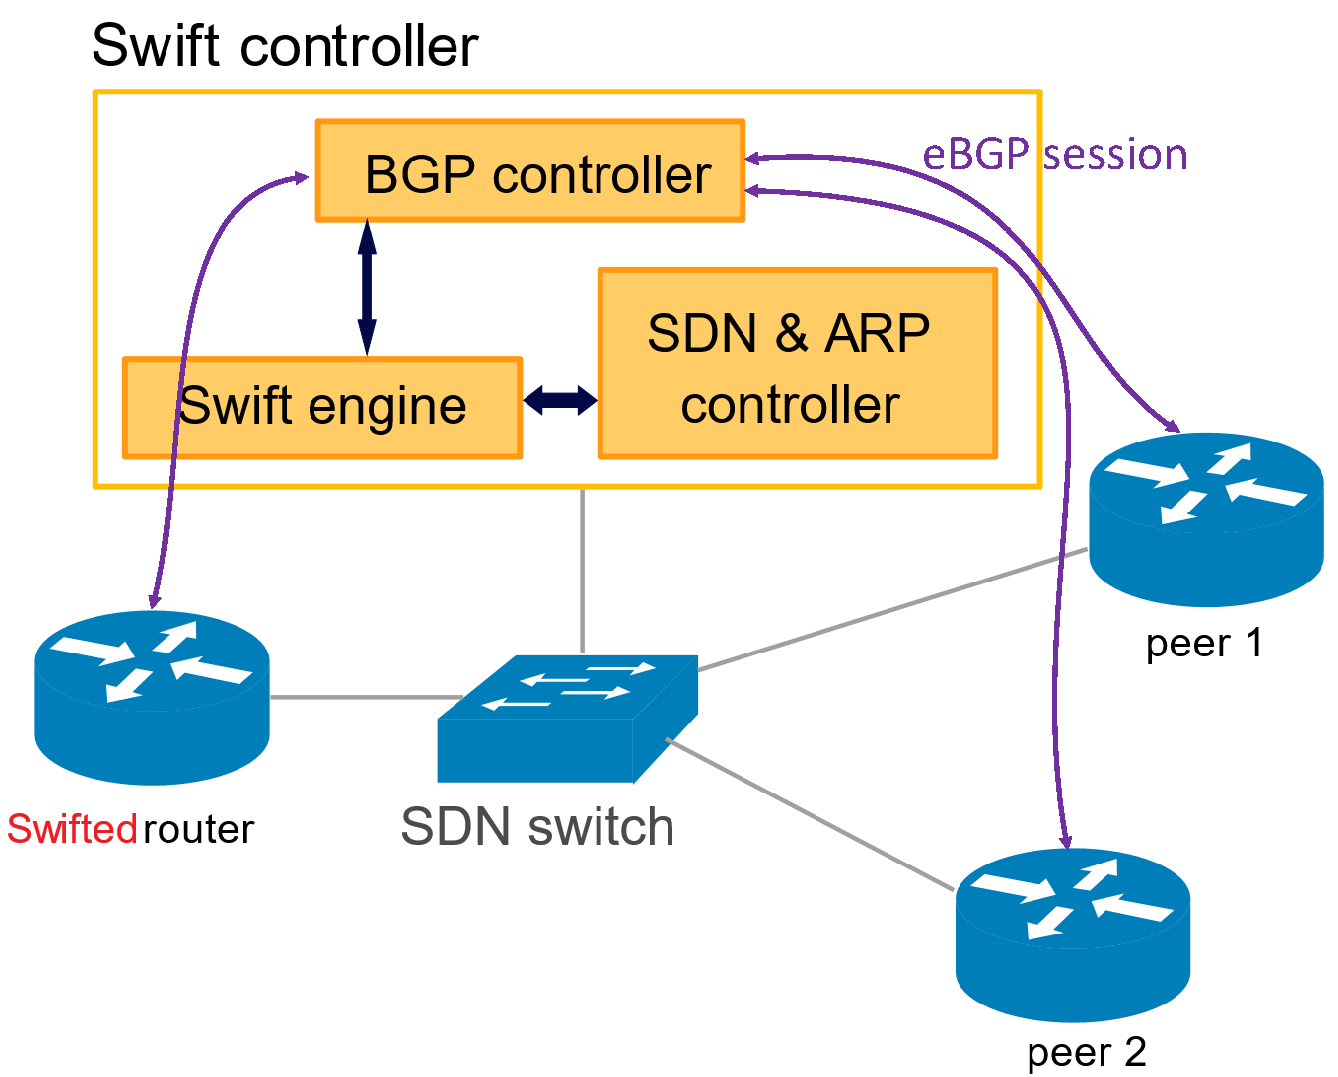
\includegraphics[scale = 0.3]{Figures/swift_topo_cropped.pdf}
\caption{Example topology of a swifted router \cite{swift}}
\end{figure}

Swift uses an SDN switch connected to the swifted router, its neighbors and to the Swift controller. The Swift Controller has three main parts, \emph{(i)} the BGP controller, \emph{(ii)} the Swift engine and \emph{(iii)} the SDN \& ARP controller. The BGP controller receives BGP updates from the peers of the swifted router. The BGP controller forwards the updates to the Swift engine. The Swift engine consists of two main modules: \emph{(i)} the burst prediction algorithm and \emph{(ii)} the encoding of routing information. These two modules are the two main features of Swift. Every peer of the swifted router has its own Swift eninge running. The SDN \& ARP controller programs flow rules into the SDN switch and manages ARP requests. 

The architecture of Swift is similar to the architecture of the iSDX. Both use a SDN switch connected to multiple BGP speaking routers, the BGP controller like the central services forwards BGP updates to the corresponding Swift engine/participant controller and every participant controller implements the functionality of the SDN \& ARP controller. 

\subsection{\label{chapter2:Swift:BPA}Burst Prediction Algorithm}
Upon remote failure the burst prediction algorithm predicts the failed AS-link. It predicts the failed link after detecting a burst. The burst is detected once a the number of received updates in a short time frame reaches a threshold.

The burst prediction algorithm takes BGP updates. It uses the updates to build a AS-topology. It also stores prefixes and the AS-path to reach these prefixes. Once a burst is triggered the burst prediction algorithm uses the received updates, stored AS-paths and the AS-topology to predict the failed AS-link.

Upon predicting a failed link the Swift Controller pushes FR flow rules into the SDN switch matching on the failed AS-link and on the corresponding backup next hop. In Figure~\ref{fig:swift_FR} the burst prediction module has predicted the AS-link 300 600 to be down. So it pushes rules matching on the AS-path 300 600 and the backup next hop in this case 400.

Every packet that traverses the failed link (has the failed AS-link in it's AS-path encoding) will get rerouted to the backup neighbor.
\begin{figure}[h]
\center
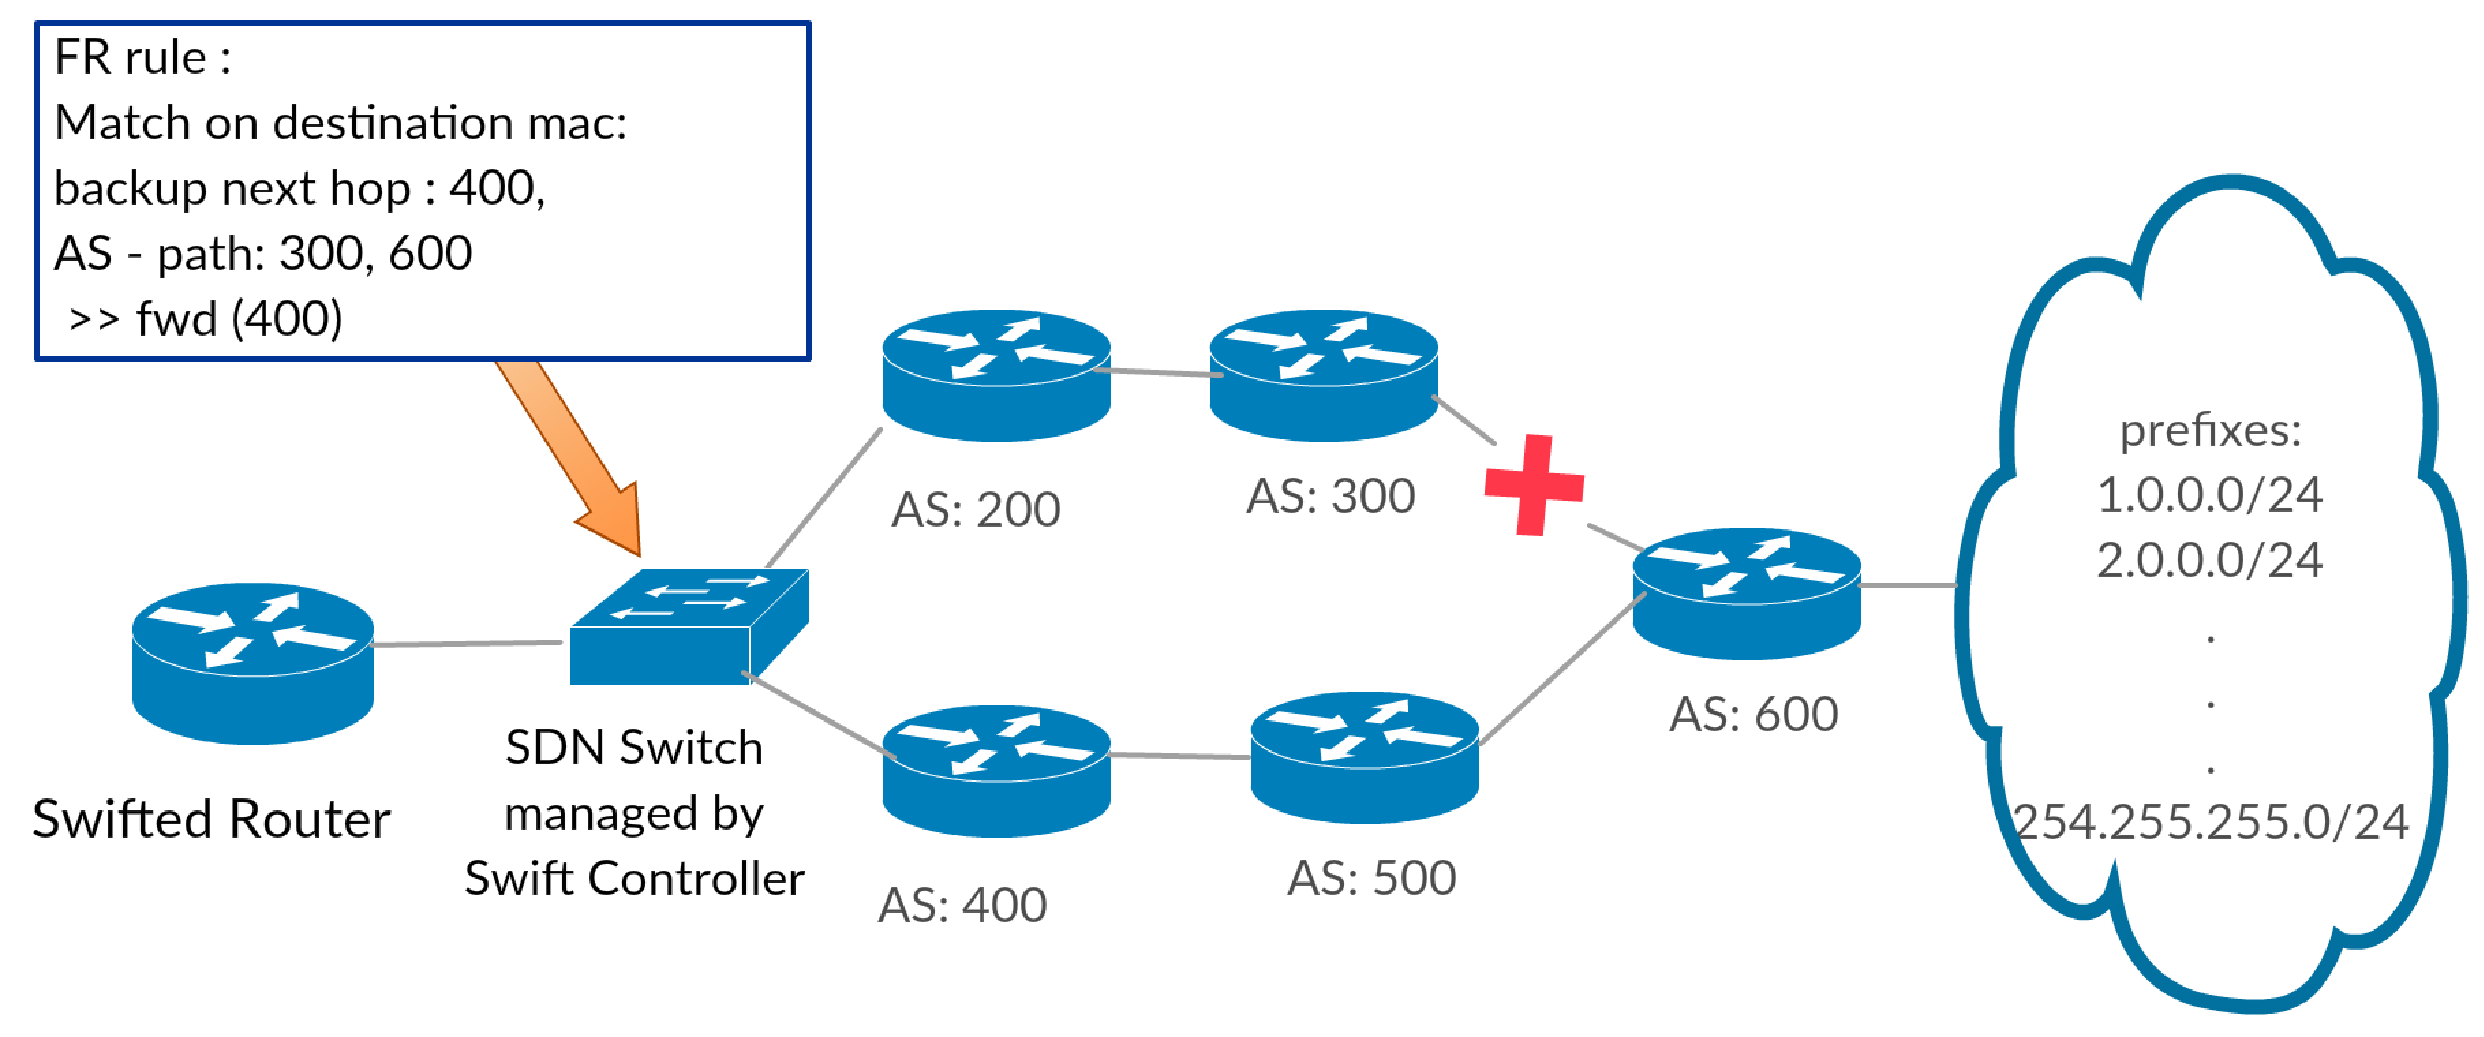
\includegraphics[scale = 0.36]{Figures/bckgrnd_swift_fr.pdf}
\caption{Example of a fast reroute}
\label{fig:swift_FR}
\end{figure}

By predicting the failed link and pushing FR rules instead of waiting for all withdrawals to arrive, Swift reduces the convergence time of the swifted router significantly.

\newpage

\subsection{\label{chapter2:Swift:encoding_of_routing_information}Encoding of Routing Information}
Swift similarly to the iSDX uses virtual next hops and the destination MAC address to encode the necessary information about the packet and its backup paths.

For every prefix Swift encodes the AS-path up to a certain depth and the backup next hops for each AS-link on that AS-path. Backup next hops are neighbors of the swifted router which also advertise the prefix and their advertised route does not traverse the specific AS-link. This encoding is then mapped to a VNH. When the swifted router wants to send a packet to any prefix it will use the VNH assigned by Swift. The VNH directly maps to the VMAC. \\
Figure~\ref{fig:swift_vmac} shows the Swifted router and the VMACs used for the prefixes advertised by the neighbors.

\begin{figure}[h]
\center
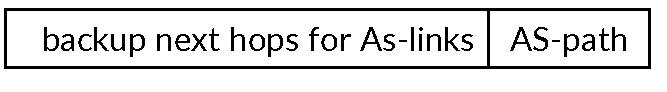
\includegraphics[scale = 0.6]{Figures/bckgrnd_swift_vmac_cropped.pdf}
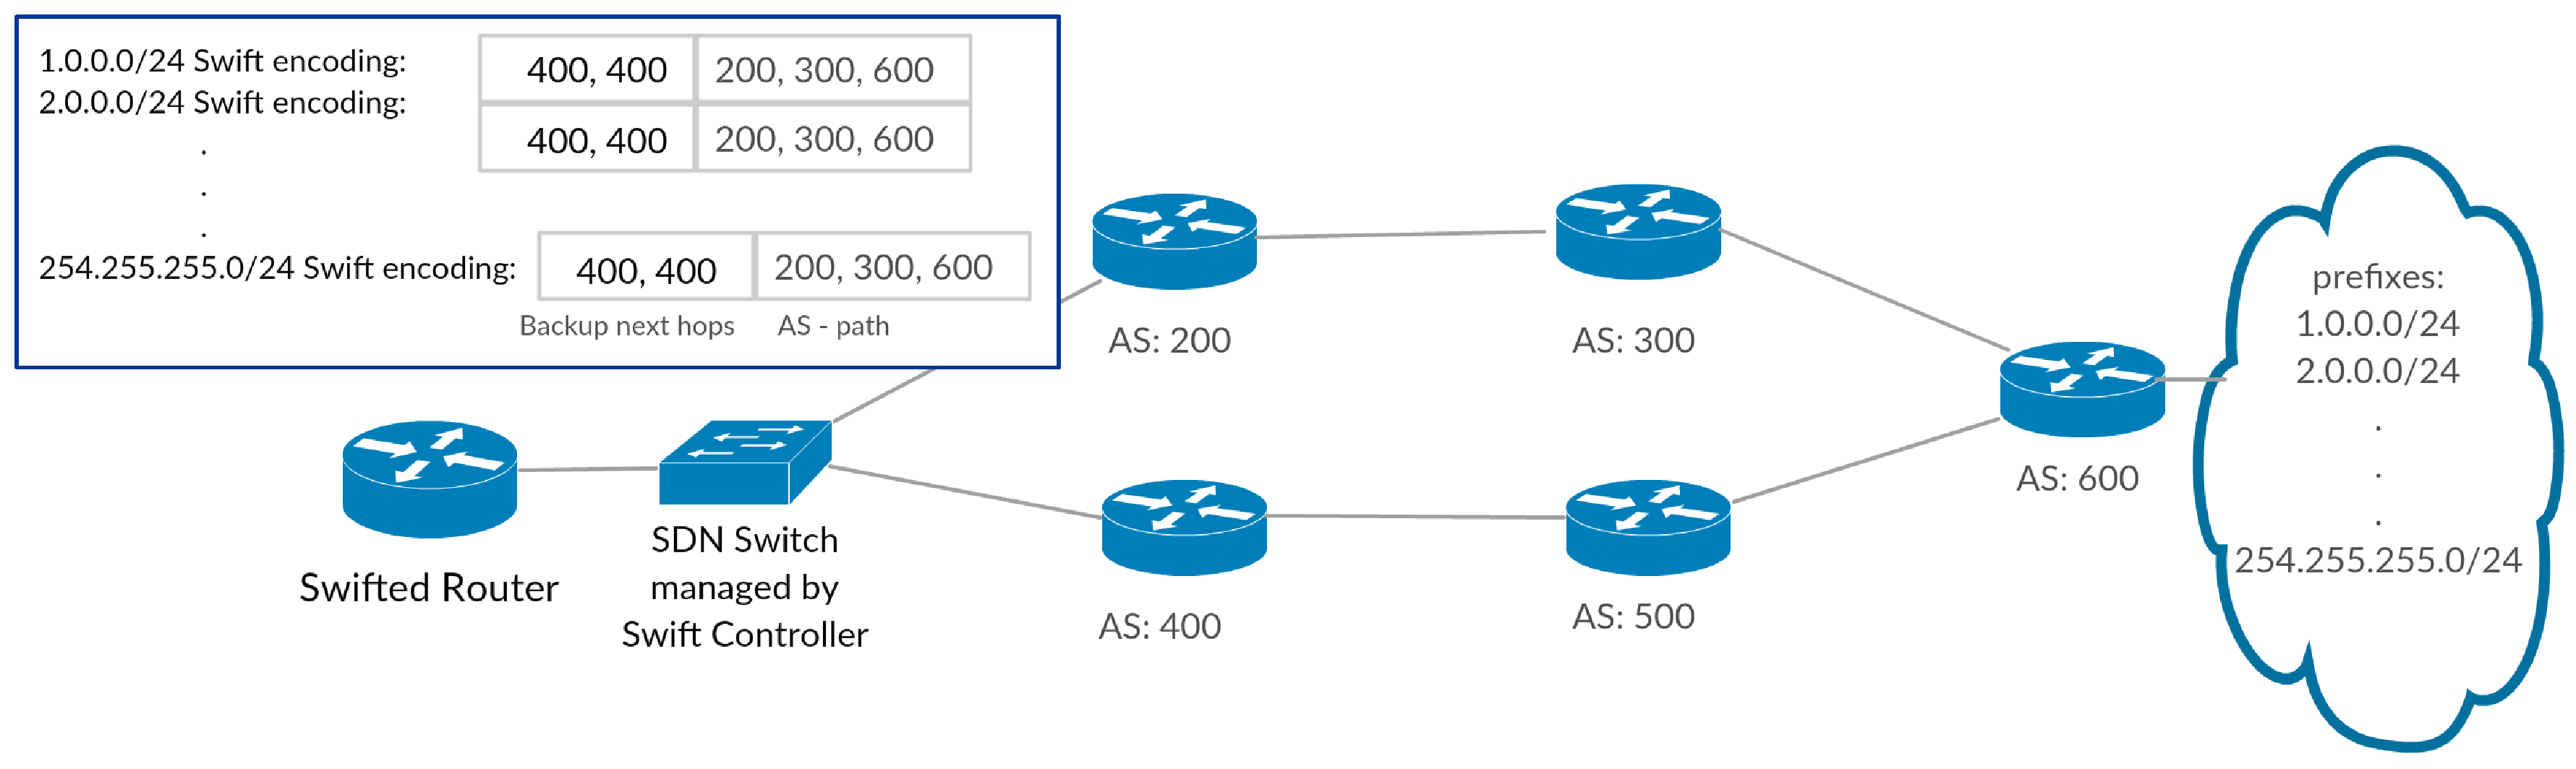
\includegraphics[scale = 0.24]{Figures/bckgrnd_swift_topology.pdf}
\caption{Example of the Swift vmac}
\label{fig:swift_vmac}
\end{figure}








